
\documentclass[12pt]{article}
\usepackage[utf8]{inputenc}
\usepackage[english]{babel}
\usepackage[a4paper, left=2 cm,right=2 cm,top=1.5 cm,bottom=1.5 cm]{geometry}
\usepackage[T1]{fontenc}
\usepackage{mathptmx}
\usepackage{mathtools}
\usepackage{gensymb}
\usepackage{graphicx}
\usepackage{enumerate}
\usepackage{cite}
\usepackage[table]{xcolor}
\usepackage{tabularx}
\newcommand\setrow[1]{\gdef\rowmac{#1}#1\ignorespaces}
\newcommand\clearrow{\global\let\rowmac\relax}
\clearrow
\usepackage{indentfirst}%wcięcie pierwszego wiersza po nagłówku

\title{%
  Cross sections for signal and background reaction}
\author{Izabela Ciepał, Joanna Kuboś, Krzysztof Nowakowski, Piotr Salabura}
\date{\today}%pusta data
% \date{\vspace{-5ex}}%usowanie daty
\begin{document}

\maketitle
\section{Signal cross-section}
\subsection{$p+p\rightarrow\Lambda (1520) +K^+ +p\rightarrow \Lambda \gamma (e^{+} + e^{-})+K^+ +p$}
An estimation of $\Lambda (1520)$ production cross-section in reaction $p+p \stackrel{E_k=4,5GeV}{\rightarrow}\Lambda (1520) + anything$ bases on the cross-section measured for $\Lambda(1115)$ production. Because of similar properties of both hyperons we assumed that only difference between production mechanism for two $\Lambda 's$ is in available phase space. Total energy required for $\Lambda (1115)$ creation is equal
\begin{equation}
  \sqrt{S_{\Lambda(1115)}}=m_p+m_K+m_\Lambda=2.55 GeV.
\end{equation}
Corresponding Value for $\Lambda(1520)$ is equal
\begin{equation}
\sqrt{S_{\Lambda(1520)}}=m_p+m_K+m_\Lambda=2.95 GeV.
\end{equation}
The difference between threshold energies for $\Lambda s$ production is 0.4 GeV, assuming similar matrix element for the production process we can estimate from fig. (\ref{fig:LambdaCS}) cross-section for inclusive $\Lambda(1520)$ production for $E_K=4,5 GeV$ ($\sqrt{S}=3.46 GeV$). $E_K=4,5 GeV$ corresponds to 0.51 GeV above the threshold for $\Lambda(1520)$, hence the available phase space corresponds to the one for $\Lambda(1115)$ production at $\sqrt S=3.06 GeV$. Using polynomial of 2-nd order to interpolate data from fig. (\ref{fig:LambdaParam}) we obtain the cross-section for inclusive $\Lambda(1115)$ production at $\sqrt{S} = 3.06 GeV$ equal  $\sigma =130 \mu b$.

\begin{figure}[]
  \label{fig:LambdaCS}
  \centering 
  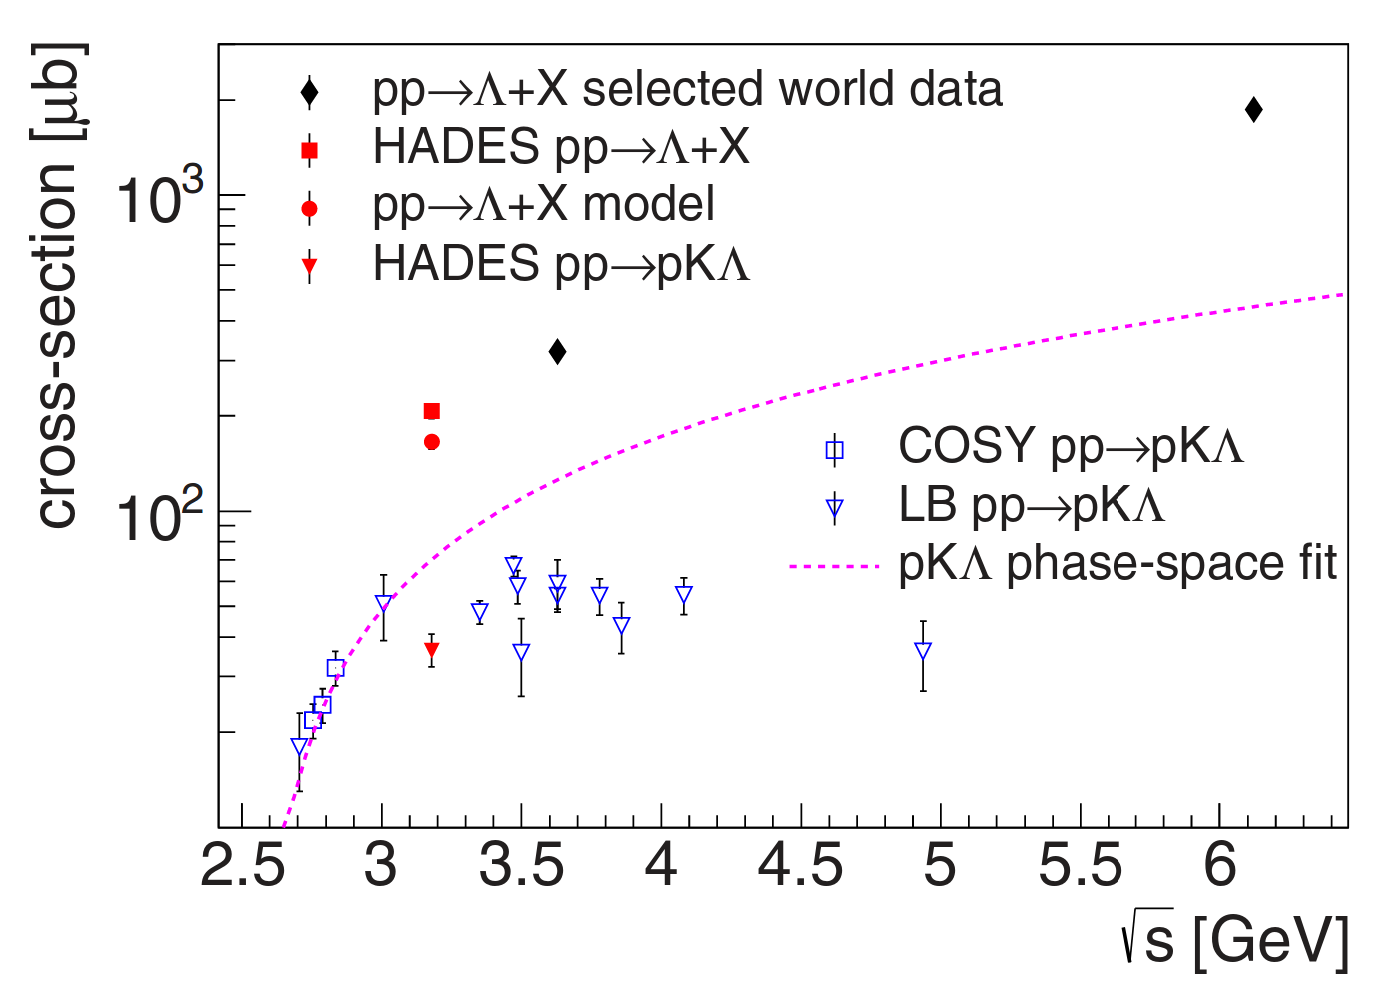
\includegraphics[width=0.8 \textwidth] {../Images/LambdaCS}
  \caption{$\Lambda$ production cross-section summary. Figure taken from \cite{Lambda3.5}.}
\end{figure}
\begin{figure}[]
  \label{fig:LambdaParam}
  \centering 
  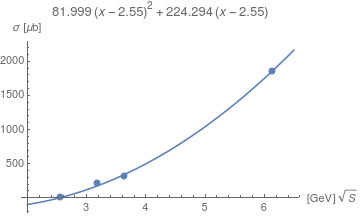
\includegraphics[width=0.6 \textwidth] {../Images/wykres}
  \caption{Parametrization of $\Lambda(1115)$ inclusive cross-section. The point (2.55,0) was fixed as a threshold energy.}
\end{figure}

\subsection{$p+p \rightarrow \Xi^- K^+ K^+ p \rightarrow \Lambda \pi^- K^+ K^+ p$}
To estimate inclusive cross-section for cascade production we have used data collected and published by HADES collaboration. The crucial point was an estimation of the ratio between $\Xi$ and $\Lambda^0$ production obtained for proton niobium experiment \cite{Ksi3.5}. This ratio is shown in fig. (\ref{fig:ratio})
. A solid line has been parameterized  by the following curve:
\begin{equation}
  \frac{\Xi}{\Lambda + \Sigma^0}=0.44 \left( 1- \left(\frac{2.2 GeV}{\sqrt{S_{NN}}} \right)^{0.027} \right)^{0.780} . 
\end{equation}
For the kinetic energy of protons $E_k=4,5 GeV$ and proton target we will get
\begin{equation}
  \frac{\Xi}{\Lambda + \Sigma^0}\stackrel{E_k=4,5GeV}{=} 0.0141.
\end{equation}

Taking from literature values of inclusive production cross-sections for $\Lambda^0$ and $\Sigma^0$ it is possible to estimate total inclusive cross-section for $\Xi^-$ production. The respective values are shown in fig (\ref{fig:crosssection}). Assuming that $\sigma_\Lambda (p=6$ GeV/c$)=\sigma_\Lambda (p=5.4$ GeV/c$)$ and following ratio between $\Sigma$ and $\Lambda$ cross-section
\begin{equation}
\frac{\sigma \Lambda^0}{\sigma \Sigma^0}\stackrel{E_k=4,5GeV}{=}3.5,
\end{equation}
a finale value is equal 
\begin{equation}
  \sigma_\Xi \approx 4.8 \mu b.
\end{equation}


\begin{figure}[]
  \centering
  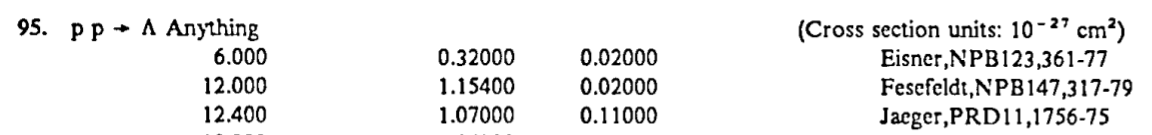
\includegraphics[width=0.8 \textwidth] {../Images/Lambda}
  \quad
  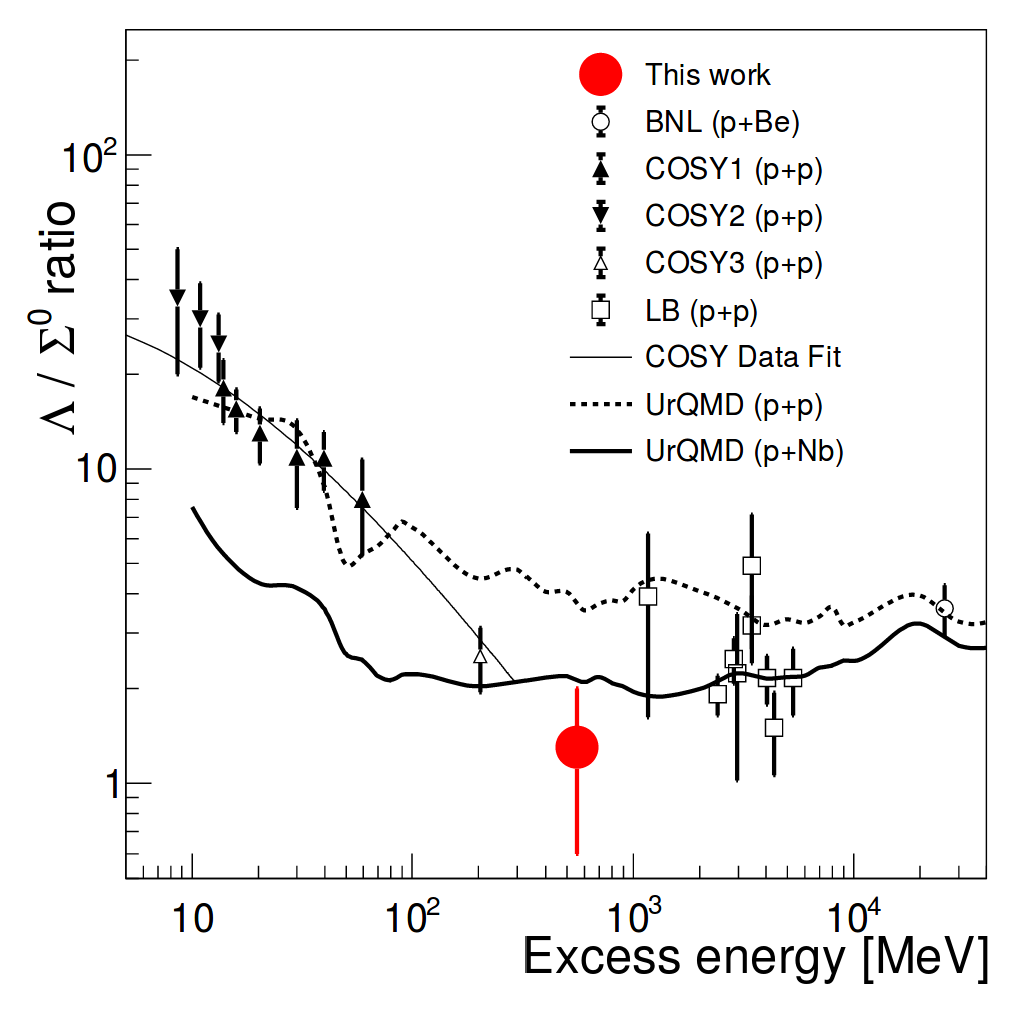
\includegraphics[width=0.5 \textwidth] {../Images/XiDoLambda}
  \caption{Cross-sections for $\Lambda^0$ (top) \cite{Bornstein} and the ratio between the cross sections for $\Sigma^0$ and $\Lambda$ (bottom) \cite{Sigma3.5} production. First table consist of four columns: beam momentum, measured cross-section, measurement error and reference to original publication. The graph shows results of measured ratio between $\Sigma^0$ and $\Lambda$ from exclusive measurements ($pp \rightarrow pK \Lambda$) and ($pp \rightarrow pK \Sigma^0$). The excess energy above production threshold refers to free nucleon-nucleon collisions.}
  \label{fig:crosssection}
\end{figure}

\begin{figure}[]
  \label{fig:ratio}
  \centering 
  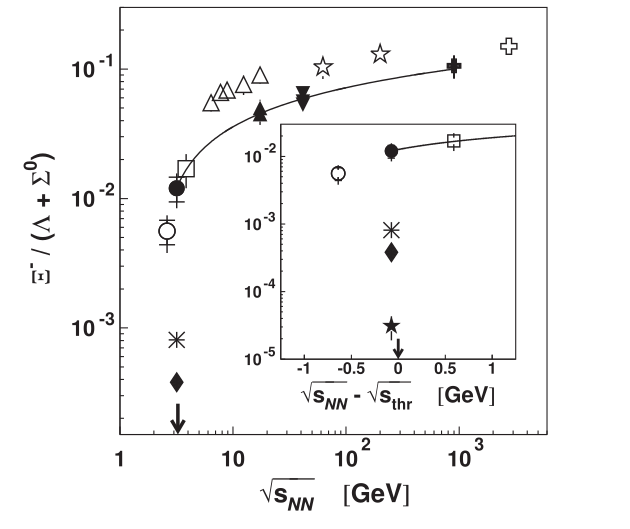
\includegraphics[width=0.8 \textwidth] {../Images/Xi}
  \caption{Ratio between $\Xi$ and $\Lambda + \Sigma$ yield \cite{Ksi3.5}.}
\end{figure}

\subsection{$\Lambda$ anisotropy}
According to HADES measurement \cite{Lambda3.5} decay yield is characterised by non-isotropic angular distribution. Results are shown in picture \ref{fig:LambdaAng}.  
\begin{figure}[]
  \label{fig:LambdaAng}
  \centering 
  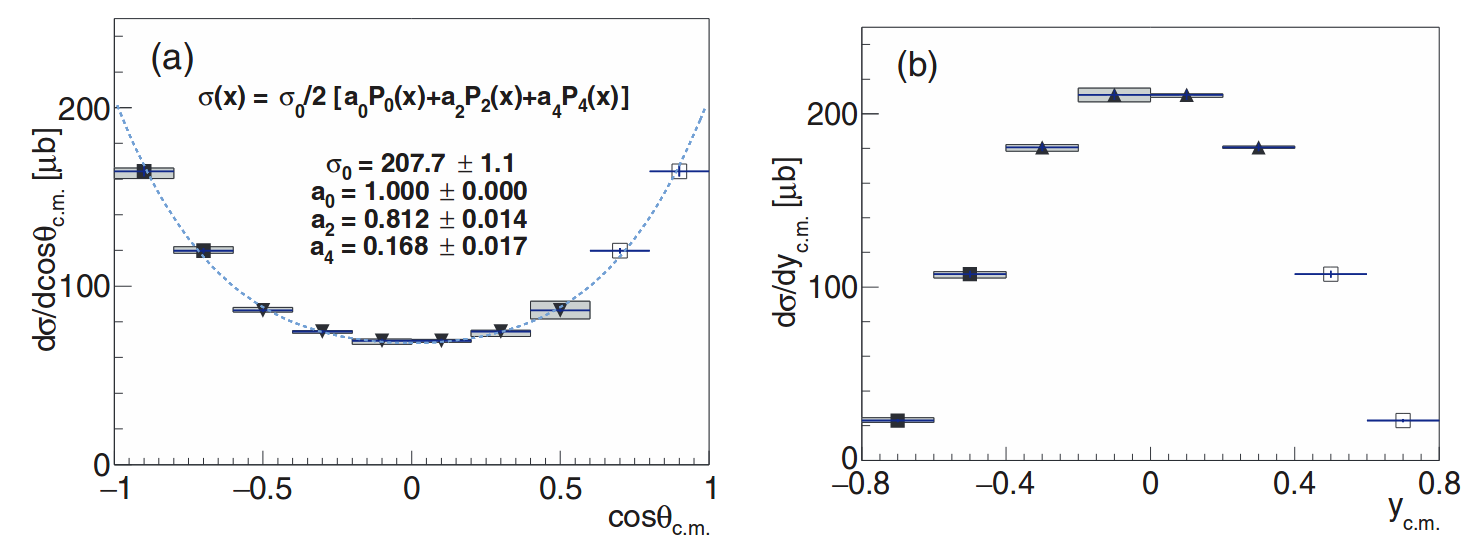
\includegraphics[width=0.8 \textwidth] {../Images/LambdaKat}
  \caption{Differential cross section distribution (a) $\frac{d\sigma}{d cos \theta_{CM}}$ and (b) $\frac{d\sigma}{d y_{CM}}$, extrapolated to the whole phase space and integrated over the $p_{CM}$ and $p_t$ variables, respectively. The full square symbols represent measured data, the empty squares refer to mirrored data, and the full triangles correspond to average between mirrored and measured data.}
\end{figure}

\newpage
\section{Background reaction}
\subsection{For channel $p+p\rightarrow\Lambda (1520) +K^+ +p\rightarrow \Lambda \gamma (e^{+} + e^{-})+K^+ +p$}

This section tries to summarise dominant sources of background. Unfortunately not all of background reactions were measured for momentum around 5.4 GeV. The relevant known cross sections (proton momentum 5.4-5.5 GeV/c) are marked by green colour. For higher momenta between 5.6 and 8 GeV/c a yellow colour was used. Reactions without any colour marking are used for much higher momenta or cases where no data is available.
\begin{enumerate}[a)]
\item $\pi^0$ Dalitz decay ($\pi^0 \rightarrow e^+ e^- \gamma =1.17 \%$)\\
  \begin{tabular}{>{\rowmac} c|c|r|>{\rowmac} r|>{\rowmac} r|>{\rowmac} r|>{\rowmac}c<{\clearrow}}
    no&reaction & cross-section & source&p[GeV/c]&$p_{thr}$[GeV/c] & L-B No.\\ 
    \hline
    \hline
    \rowcolor{green!60}
    \setrow{\bfseries}
    1&pp $\pi^+ \pi^- \pi^0$& 1.84 mb & \cite{Bornstein} &5.5&1.60&169\\
    \setrow{\bfseries}
    2&pp $\pi^+ \pi^- 2 \pi^0$ & 0.3 mb& similar to 2.2 a) 1.& & &\\
    \setrow{\bfseries}
    3&pp $\pi^+ \pi^- 3 \pi^0$ & 0.1 mb& similar to reaction no 5& & &\\
    4&pn $2\pi^+ \pi^- \pi^0$ & 0.3 mb& similar to 2.2 a) 1.& & &\\
    \rowcolor{green!60}
    5&pp $2\pi^+ 2\pi^- \pi^0$& $88.0 \mu b$ &\cite{Bornstein}&5.5&2.41&179\\
    6&pp $3\pi^+ 3\pi^- \pi^0$& $20 \mu b$&\cite{Bornstein}&8.80&3.26&185\\
    \rowcolor{red!35}
      &total:&2.24 mb &
  \end{tabular}
  
\item Reaction with $\Lambda$ and di-lepton source (BR: $\pi^0 \rightarrow e^+e^- \gamma=1.17\%$). \\
  \begin{tabular}{>{\rowmac}c|c|r|>{\rowmac} p{3.5 cm}|>{\rowmac} r|>{\rowmac} r|>{\rowmac}c<{\clearrow}}
    no&reaction & cross-section & source &p[GeV/c]& $p_{thr}$[GeV/c] & L-B No.\\ 
    \hline
    \hline
    \rowcolor{green!60}
    \setrow{\bfseries}1&p $\Lambda K^+ \pi^0$& $43 \mu b$& \cite{Bornstein}& 5.4& 2.74&83\\
    2&n $\Lambda K^+ \pi^+\pi^0$& $20 \mu b$& & & &\\
    3&p $\Lambda K^+ 2 \pi^0$& $10 \mu b$& & & &\\
    \setrow{\bfseries}
    4&p $\Lambda K^0 \pi^+ 2\pi^0$& $7 \mu b$& & & &\\
    \rowcolor{green!60}
    \setrow{\bfseries}
    5&p $\Lambda K^0 \pi^+ \pi^0$& $17 \mu b$& \cite{Bornstein}&5.5&3.182&78\\
    6&p $\Lambda K^+ 3 \pi^0$& $7 \mu b$& & & &\\
    \rowcolor{yellow!50}
    7&p $\Lambda \pi^+ \pi^0 \pi^- K^+$& $14.2 \mu b$ & \cite{Bornstein} & 6.92 &3.62&77 \\    
    \rowcolor{green!60}
    \setrow{\bfseries}
    8&p $ K^+ \Lambda (1520) \rightarrow \Lambda 2 \pi^0$ & BR $\approx 3 \%$ & calculated from C-G coefficients for decay into two pions & & & \\
    \rowcolor{red!35}
      &total:& &
  \end{tabular}

\item Reaction with $\Sigma^0$ (BR: $\Sigma^0 \rightarrow \Lambda e^+ e^- =5 \cdot 10^{-3}$, $\Sigma^0 \rightarrow \gamma \Lambda^0 \approx 100\% $ )\\
  \begin{tabular}{>{\rowmac} c|c|r|>{\rowmac} r|>{\rowmac} r|>{\rowmac} r|>{\rowmac}c<{\clearrow}}
    no&reaction & cross-section & source &p[GeV/c]&$p_{thr}$[GeV/c] & L-B No.\\ 
    \hline
    \hline
    1&p $\Sigma^0 K^+ \pi^0$& $18 \mu b$& similar to reaction no 4\\
    \rowcolor{green!60}
    \setrow{\bfseries}2&p $\Sigma^0 K^+$ & $27 \mu b$& \cite{Bornstein}&5.4&2.67&108\\
    \rowcolor{yellow!50}
    3&p $\Sigma^0 K^+ \pi^+ \pi^-$& $13.7 \mu b$& \cite{Bornstein}& 6.92 &3.43 &106\\
    \rowcolor{green!60}
    \setrow{\bfseries}
    4&p $\Sigma^0 K^0 \pi^+$& $18 \mu b$& \cite{Bornstein}&5.4&3.00&107\\
    \rowcolor{red!35}
      &total:&$45 \mu b$ &
  \end{tabular}

\item Reaction with $\Sigma^-$ (BR: $\Sigma^- \rightarrow n \pi^- =99.9\% $)\\
  \begin{tabular}{>{\rowmac} c|c|r|>{\rowmac} r|>{\rowmac} r|>{\rowmac} r|>{\rowmac}c<{\clearrow}}
    no&reaction & cross-section & source&p[GeV/c]&$p_{thr}$[GeV/c] & L-B No.\\ 
    \hline
    \hline
    \rowcolor{yellow!50}
    1&p $\Sigma^- K^+ \pi^0 \pi^+$& $22 \mu b$& \cite{Bornstein}&7.87&3.43&110\\
    2&p $\Sigma^- K^0 \pi^0 2\pi^+$& $13 \mu b$& \cite{Bornstein}&10&3.90&112\\
    \rowcolor{red!35}
      &total:& 0&
  \end{tabular}
\end{enumerate}
\subsection{For channel$p+p \rightarrow \Xi^- K^+ K^+ p \rightarrow \Lambda \pi^- K^+ K^+ p$}  
\begin{enumerate}[a)]
\item Two $\pi^-$ production\\
  \begin{tabular}{>{\rowmac} c|c|r|>{\rowmac} r|>{\rowmac} r|>{\rowmac} r|>{\rowmac}c<{\clearrow}}
    no&reaction & cross-section & source &p[GeV/c]&$p_{thr}$[GeV/c] & L-B No.\\ 
    \hline
    \hline
    \rowcolor{green!60}
    \setrow{\bfseries}
    1&pp $2\pi^+ 2\pi^-$& $227 \mu b$&\cite{Bornstein}&5.50&2.016&182\\
    2&pp $2\pi^+ 2\pi^- \pi^0$& $88 \mu b$& \cite{Bornstein}& 5.5 & 2.41 & 179\\
    \rowcolor{green!60}
    \setrow{\bfseries}
    3&pn $3\pi^+ 2\pi^-$& $98 \mu b$&\cite{Bornstein}&5.5&2.428&130\\
    \rowcolor{red!35}
      &total:&$325 \mu b$ &
  \end{tabular}
\item $\Lambda$ production associated with $\pi^-$\\
  \begin{tabular}{>{\rowmac} c|c|r|>{\rowmac} r|>{\rowmac} r|>{\rowmac} r|>{\rowmac}c<{\clearrow}}
    no&reaction & cross-section & source& p[GeV/c]& $p_{thr}$[GeV/c] & L-B No.\\ 
    \hline
    \hline
    \rowcolor{green!60}
    \setrow{\bfseries}
    1&p $\Lambda K^0 \pi^+$& $60 \mu b$& \cite{Bornstein}&5.4&2.766&80\\
    \rowcolor{green!60}
    \setrow{\bfseries}
    2&p $\Lambda K^0 \pi^+ \pi^0$& $17 \mu b$& \cite{Bornstein}& 5.5 &3.182&78\\
    \rowcolor{yellow!50}
    3&n $\Lambda K^0 2 \pi^+$& $29.6 \mu b$& \cite{Bornstein}&6.920&3.204&88\\
    \rowcolor{yellow!50}
    4&p $\Lambda \pi^+ \pi^0 \pi^- K^+$& $14.2 \mu b$& \cite{Bornstein}&6.92&3.62&77\\
    \rowcolor{green!60}
    \setrow{\bfseries}
    5&p $\Lambda \pi^+ \pi^- K^+$& $21.3 \mu b$& \cite{Bornstein}&5.5&3.19&79\\
    6&p $\Lambda 2 \pi^+ \pi^- \pi^0 K^0$& $34.0 \mu b$& \cite{Bornstein}&10&4.10&81\\
    \rowcolor{yellow!50}
    7&p $\Lambda 2 \pi^+ \pi^- K^0$& $6.2 \mu b$& \cite{Bornstein}&6.92&3.65&82\\
    \rowcolor{yellow!50}
    8&n $\Lambda 2 \pi^+ \pi^- K^+$& $10.1 \mu b$& \cite{Bornstein}&6.92&3.64&87\\
    9&n $\Lambda 3 \pi^+ \pi^- K^0$& $13.0 \mu b$& \cite{Bornstein}&10&4.12&89\\
    \rowcolor{red!35}
      &total:&$98 \mu b$ &
  \end{tabular}

\item $\Sigma^0$ production associated with $\pi^-$ (BR:$\Sigma^0 \rightarrow \Lambda^0 \approx 100\% $, BR:$K^0_s \rightarrow \pi^+ \pi^- =69.20 \% $)\\
  \begin{tabular}{>{\rowmac}c|c|r|>{\rowmac} p{3.5 cm}|>{\rowmac} r|>{\rowmac} r|>{\rowmac}c<{\clearrow}}
    no&reaction & cross-section & source& p[GeV/c]& $p_{thr}$[GeV/c] & L-B No.\\ 
    \hline
    \hline
    \rowcolor{green!60}
    \setrow{\bfseries}
    1&p $\Sigma K^0 \pi^+$& $18 \mu b$& \cite{Bornstein}&5.4&2.998&107\\
    \rowcolor{yellow!50}
    2&p $\Sigma \pi^+ \pi^- K^+$& $13.7 \mu b$& \cite{Bornstein}&6.92&3.43&106\\
    \rowcolor{green!60}
    3&n $\Sigma K^0 2 \pi^+$& $6.6 \mu b$& ratio between b.1 and b.3 reaction\\
    \rowcolor{red!35}
      &total:&$ 18 \mu b$ &
  \end{tabular}

\item $K^0$ production (BR:$K^0_s \rightarrow \pi^+ \pi^- =69.20 \% $)\\
  \begin{tabular}{>{\rowmac} c|c|r|>{\rowmac} r|>{\rowmac} r|>{\rowmac} r|>{\rowmac}c<{\clearrow}}
    no&reaction & cross-section & source& p[GeV/c]& $p_{thr}$[GeV/c] & L-B No.\\ 
    \hline
    \hline
    \rowcolor{yellow!50}
    1& $\Sigma^+ p \pi^+ \pi^- K^0$&$10.5 \mu b$& \cite{Bornstein}& 6.92&3.43 &96\\
    \rowcolor{yellow!50}
    2& $n p \pi^+ \pi^- K^0 K^+$&$5.4 \mu b$& \cite{Bornstein}& 6.92&4.24 &125\\
    3& $n p 2 \pi^+ \pi^- 2 K^0$&$36.0 \mu b$& \cite{Bornstein}& 10&4.75 &128\\
    \rowcolor{yellow!50}
    4& $2 p 2 \pi^+ \pi^- 2 K^0$&$6.3 \mu b$& \cite{Bornstein}& 7.87&4.25 &175\\
    \rowcolor{yellow!50}
    5& $2 p \pi^- K^0 K^+$ & $16 \mu b$& \cite{Bornstein}& 6.92&3.77 &195\\
    \rowcolor{green!60}
    6&$2 p 2 K^0$ & $6.4 \mu b$&\cite{Bornstein}&5.5&3.32&201\\
    \rowcolor{yellow!50}
    7&$n p \pi^+ 2 K^0$ & $15.7 \mu b$&\cite{Bornstein}&6.92&3.78&126\\
    \rowcolor{red!35}
      &total:& 0  &
  \end{tabular}
\end{enumerate}
  
\bibliographystyle{utphys}
\bibliography{../Bibliografia/bibliografia}{}

\end{document}

\grid